%% ------------------------------------------------------------------------- %%
\chapter{Introdução}
\label{cap:introducao}

O rápido  desenvolvimento de sistemas de transporte e crescimento das cidades
tem sido acompanhado de fluxos de deslocamento cada vez mais complexos e
volumosos, aumentando também os desafios para as questões de mobilidade urbana. 
\cite{Zhang2011} mostram em seu estudo uma estimativa de que cerca de 40\% da população mundial passa pelo menos uma
hora no trânsito todos os dias \citep{Zhang2011}. Os impactos negativos de
uma infraestrutura de transporte ineficiente também geram perdas econômicas,
como mostra um estudo de X, que calcula que
os gargalos em mobilidade no Brasil geram prejuízos de R\$ xxxx milhões de
reais anualmente. Tais dados mostram como ainda existe espaço para se buscar
melhorias para os sistemas de transporte, de maneira
a melhorar a qualidade de vida dos cidadãos e reduzir custos.

Para isso, a tecnologia tem sido amplamente empregada como um agente
facilitador de coleta e disponibilização de várias fontes de informação que
permitem cidadãos, pesquisadores, empresas e agentes públicos a realizarem
estudos para entender problemas de mobilidade urbana e buscarem soluções.
Várias tipos de dados podem ser coletados de diferentes fontes, como sensores
de GPS, câmeras de tráfego, e mesmo coletados manualmente. Na administração
pública, essas fontes de informação podem ser utilizadas para prover serviços
melhores para a população, melhorar a gestão da infraestrutura urbana e dar
suporte para a tomada de decisão baseada em evidências. [1, 2].  Dentro desse
contexto, nós focamos nosso estudo em dados de mobilidade urbana da região
metropolitana de S\~ao Paulo (RMSP).

A cada dez anos, desde 1967, a Companhia Metropolitano de São Paulo (Metrô),
que gerencia o sistema de metrô da cidade, conduz um estudo censitário de
mobilidade chamado \emph{Pesquisa Origem-Destino} (OD). A pesquisa OD é feita
através de entrevistas aos cidadãos e coleta dados sobre suas vidas e
atividades de deslocamento em um dia típico de trabalho. O resultado é um amplo
panorama social e de mobilidade da população na RMSP. A última pesquisa OD
(2017) mostra que ocorrem cerca de 42 milhões de deslocamentos nas 24 horas de
um dia comum de trabalho. Além das informações de origem (O) e destino (D), a
pesquisa coleta informações socioeconômicas dos cidadãos e também outros dados
sobre os deslocamentos, como o modo de transporte utilizado, o motivo da
viagem, idade, gênero, renda familiar. Com isso, a pesquisa OD se traduz num
grande conjunto de dados com múltiplos atributos.

Embora a pesquisa OD mencionada seja bem abrangente e precisa, 
os gestores precisam de ferramentas adequadas para analisar esta grande quantidade de
dados multivariados. O uso de planilhas e gráficos com informações agregadas
ajudam a compreendê-los, mostrando, por exemplo, o número de usuários 
do sistema de transporte público ao longo dos anos, ou o número de homens ${X}$ mulheres
que saem diariamente a trabalho. Técnicas de visualização, como mapas de densidade,
podem ajudar a responder questões geoespaciais, como encontrar regiões que concentram
os maiores fluxos de mobilidade durante o dia ou quais os pares de origem e destino
mais comuns. No entando, considerando a grande quantidade de dados (e atributos) gerados
nas cidades, traduzir dados geolocalizados em imagens significativas é um greande desafio.

Um estudo recente sobre métodos de visualização de fluxos de mobilidade indica um
uso comun de visualizações baseadas em linhas para estudar a estrutura desses dados,
o que geralmente inclui descoberta de padrões e agrupamentos \cite{Chen2015}. Cores e texturas
podem ser utilizados para dar informações adicionais sobre os objetos estudados, como sua velocidade, direção,
meio de transporte utilizado, etc. Porém, desenhar diretamente linhas das trajetórias em um mapa
torna-se pouco efetivo em cenários com uma grande quantidade de dados. Uma visualização das 42 milhões de trajetórias,
como os registrados pela última pesquisa OD, resulta em uma imagem completamente ofuscada
pela sobreposição e cruzamento dos fluxos, como mostra a Figura \cite{fig:cluttered-graph}.
Para isso, técnicas de \emph{bundling} aprimoram as visualizações baseadas em linha e podem
representar grandes volumes de dados de trajetórias.

Bundling techniques improve upon line-based techniques and can
depict high volumes of trajectory data by essentially simplifying trajectories in the
image space, grouping spatially close and data-wise similar trajectories together [7,
8].


\begin{figure}[!htb]
  \centering
  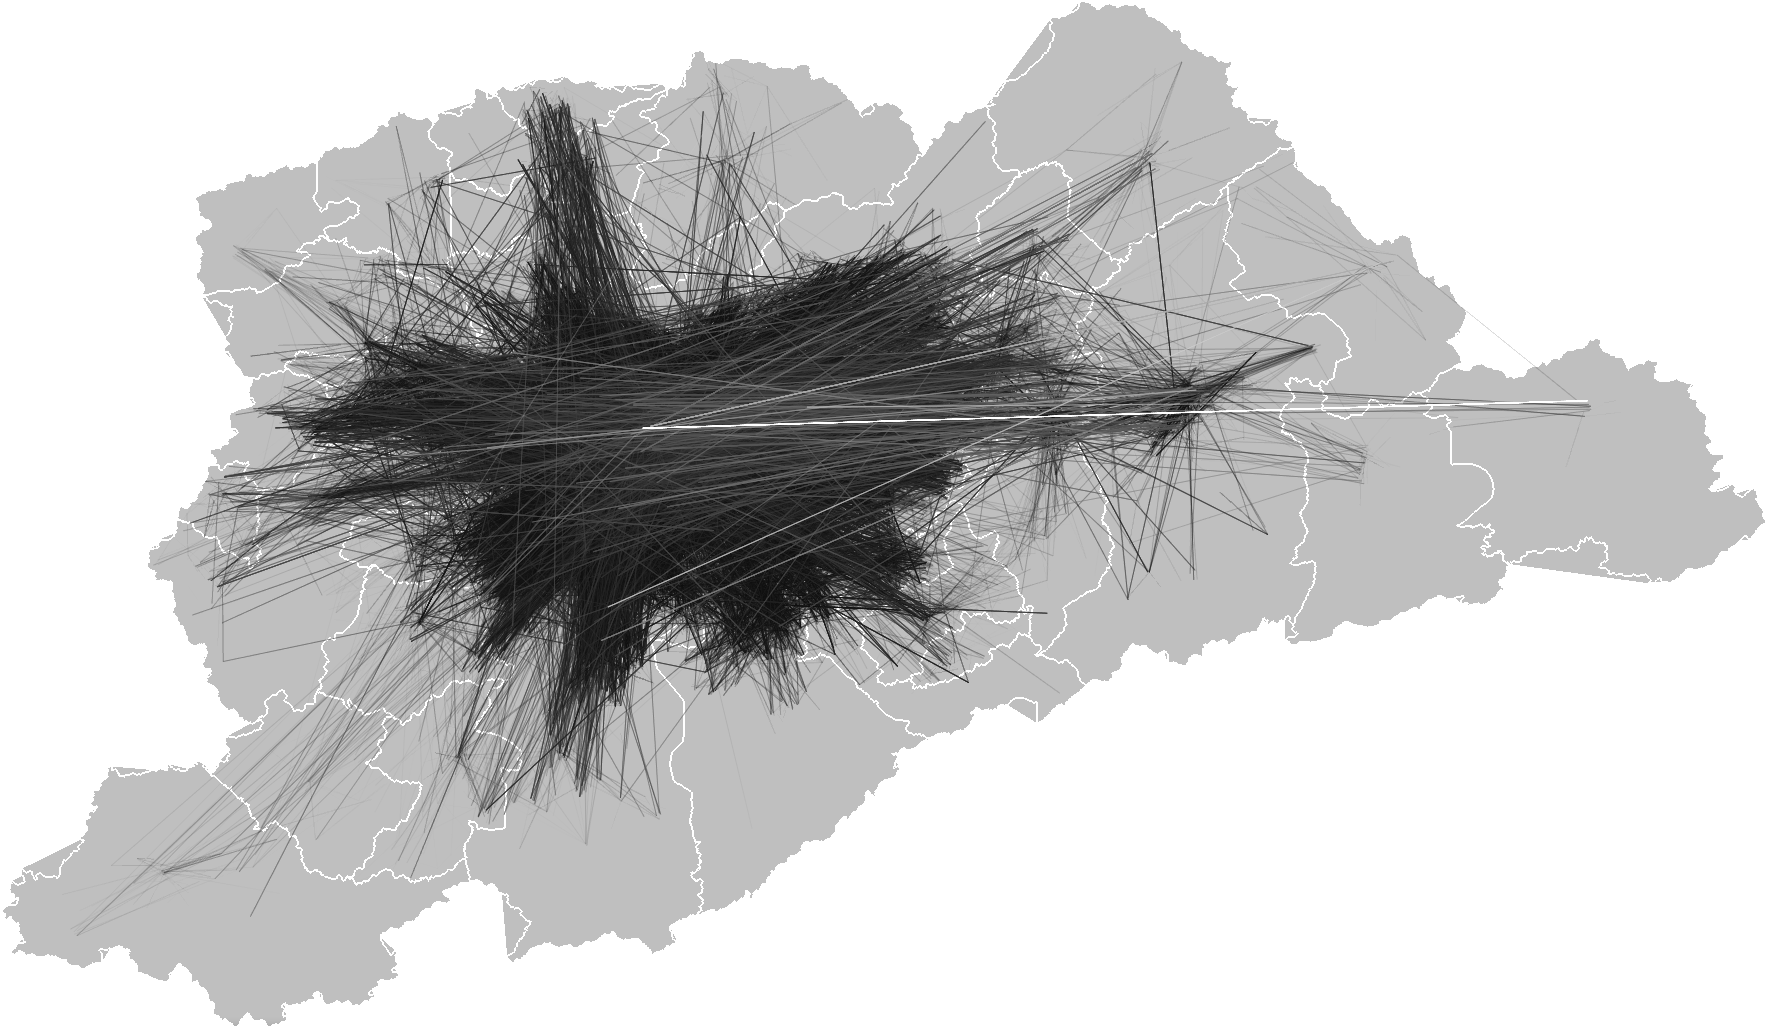
\includegraphics[width=150mm]{../figuras/unbundled-edges+grayscale+512px.png}
  \caption[Trajetórias da pesquisa OD na região metropolitana de S\~ao Paulo]{Trajetórias da pesquisa
OD na região metropolitana de S\~ao Paulo. \label{fig:cluttered-graph}}

\end{figure}

Neste trabalho nos propomos o uso de um conjunto de técnicas de visualização
para explorar as características de uma grande quantidade de dados de
mobilidade urbana. Para isso, nós adaptamos uma técnica que revelou resultados
interessantes na visualização de trajetórias em outros cenários como o do
tráfego aéreo e rastreamento do movimento da visão para o nosso contexto.
Nosso estudo permitiu a visualização dos dados em diferentes níveis de
granularidade espaço temporal, ajudando a encontrar padrões de mobilidade e
revelar novos insights a respeito do sistema de transporte de S\~ao Paulo e da
infraestrutura da cidade. Em contraste a outros trabalhos que utilizam técnicas
similares, nossa pesquisa ainda se destaca pela grande quantidade de dados
analisada. Para isso, apresentamos também uma metodologia para reduzir o tamanho
do conjunto de dados com impacto mínimo na sua significância estatística.
